\documentclass[portuguese,10pt,3col]{cheatsheet}

% Set cheat sheet information
\setcheatsheettitle{\textbf{Formulário de \textcopyright ontrolo \bishop}}
\setcheatsheetversion{v3.0}
\setcheatsheetdate{15/07/2022}
\setcheatsheetauthor{João Marafuz Gaspar -- 96240}
\setcheatsheetinstitution{IST, 2022}
\setcheatsheetsource{Formulário de Henrique Alves Pocinho -- 99952 e Maria Madalena Barros -- 100026}

% Custom commands
\makeatletter
\newcommand*\bigcdot{\mathpalette\bigcdot@{.5}}
\newcommand*\bigcdot@[2]{\mathbin{\vcenter{\hbox{\scalebox{#2}{$\m@th#1\bullet$}}}}}
\makeatother

\begin{document}

{\huge
\begin{center}
    \textbf{Formulário de \textcopyright ontrolo \bishop} \footnotesize \textcolor{bblue}{\texttt{[v1.0 - 2022-07-15]}}
\end{center}
}

\begin{multicols}{3}

%------------ Modelação ---------------
\begin{cheatsheetbox}{Modelação}{-0.3cm}
    \begin{tabular}{l c c}
        Mola & $F_s = -kx$ & $T_s = -k\theta$ \\
        Atrito & $F_a = -\beta \dot{x}$ & $T_a = -\beta\dot{\theta}$ \\
        Lei de Newton & $\sum F =\frac{d}{dt}\left(m \dot{x}\right)$ & $\sum F = \frac{d}{dt}(J \dot{\theta})$
    \end{tabular} \\
    
    \textbf{Linearização} de $\dot{y}(t) = f\left(y(t), u(t)\right)$:
    \begin{enumerate}
        \item Equilíbrio -- $\dot{y}(t) = 0 \Leftrightarrow \left\{(y_0, u_0): f(y_0, u_0) = 0\right\}$
        \item Aprox. lin. -- $\dot{y} = f(y_0, u_0) + \frac{\partial f}{\partial y}\big|_\text{eq} (y - y_0) + \frac{\partial f}{\partial u}\big|_\text{eq} (u - u_0)$
        \item Sistema linearizado -- $\boxed{\delta\dot{y} = a\delta y + b \delta u}$
    \end{enumerate}
\end{cheatsheetbox}

\begin{cheatsheetbox}{Resposta no Tempo}{0.0cm}
    \begin{tabular}{c c c}
	    $x(t) = TL^{-1}\left\{X(s)\right\}$ & $\Longleftrightarrow$ & $X(s) = \int_0^\infty x(t)e^{-st} dt$ \\
	    $\delta(t \mathbin{\textcolor{bblue}{-}} \textcolor{bblue}{t_0})$ & $\Longleftrightarrow$ & $1 \times \textcolor{bblue}{e^{-st_0}}$ \\
	     \vspace{0.1cm}
	    $t^n \textcolor{bblue}{e^{-\alpha t}} u(t)$ & $\Longleftrightarrow$ & $\displaystyle \frac{n!}{(s \mathbin{\textcolor{bblue}{+}} \textcolor{bblue}{\alpha})^{n+1}}$ \\
	    \vspace{0.1cm}
	    $\textcolor{bblue}{t} \textcolor{oorange}{e^{-\alpha t}} \sin(\beta t) u(t)$ & $\Longleftrightarrow$ & $\displaystyle \frac{\textcolor{bblue}{2}\beta \textcolor{bblue}{(s} \mathbin{\textcolor{bblue}{+}} \textcolor{bblue}{\alpha)}}{\textcolor{bblue}{\left[\textcolor{black}{(s} \mathbin{\textcolor{oorange}{+}} \textcolor{oorange}{\alpha}\textcolor{black}{)^2} \mathbin{\textcolor{black}{+}} \textcolor{black}{\beta^2}\right]^{\textcolor{bblue}{2}}}}$ \\
	    \vspace{0.1cm}
	    $\textcolor{bblue}{t} \textcolor{oorange}{e^{-\alpha t}} \cos(\beta t) u(t)$ & $\Longleftrightarrow$ & $\displaystyle \frac{\textcolor{bblue}{(} s \mathbin{\textcolor{oorange}{+}} \textcolor{oorange}{\alpha}\textcolor{bblue}{)^2} \mathbin{\textcolor{bblue}{-}} \textcolor{bblue}{\beta^2}}{\textcolor{bblue}{\left[\textcolor{black}{(s} \mathbin{\textcolor{oorange}{+}} \textcolor{oorange}{\alpha}\textcolor{black}{)^2} \mathbin{\textcolor{black}{+}} \textcolor{black}{\beta^2}\right]^{\textcolor{bblue}{2}}}}$ \\
	    $x(at)$ & $\Longleftrightarrow$ & $\frac{1}{a}X(s/a), \ a > 0$ \\
	    $x(t - t_0)u(t - t_0)$ & $\Longleftrightarrow$ & $e^{-st_0}X(s) , \ t_0 > 0$ \\
	    $\displaystyle \frac{dx(t)}{dt}$ & $\Longleftrightarrow$ & $sX(s) - x(0^-)$ \\
	    $\int_0^tx(\tau)d\tau$ & $\Longleftrightarrow$ & $X(s)/s$
	\end{tabular} \\
	
	\textbf{TVI:} $\displaystyle x(0^+) = \lim_{t \to 0}x(t) = \lim_{s \to \infty}sX(s)$ \\
	\textbf{TVF:} $\displaystyle x(\infty) = \lim_{t \to \infty}x(t) = \lim_{s \to 0}sX(s)$ se todos os pólos de $sX(s)$ estiverem no s.p.c.e.\\
	
	Função transf. \textbf{própria}: $G(s) = \frac{N(s)}{D(s)} = \frac{\text{grau } m}{\text{grau } n}, \ n \geq m$ \\
	
	SLIT 1ª ordem: \\ $\dot{y}(t) = a\left[k_0 r(t) - y(t)\right] \stackrel{TL}{\rightarrow} Y(s) = \frac{1}{s + a}y(0^-) + k_0 \frac{a}{s + a}R(s) \\ \stackrel{TL^{-1}}{\longrightarrow} y(t) = e^{-at}y(0^-) + k_0\left(1 - e^{-at}\right)u(t)$ \\
	Ganho estático: $\lim_{s \to 0} G(s) = k_0$ \\
	Tempo de estab. $\mu \%$: $e^{-at_s } = \mu \% \Leftrightarrow t_s(\mu \%) = \frac{\ln(\mu / 100)}{-a}$ \\
	SLIT 2ª ordem: $G(s) = \frac{\omega_n^2}{s^2 + 2\zeta \omega_n s + \omega_n^2}$ \\
	$s^2 + 2\zeta \omega_n s + \omega_n^2 = 0 \Leftrightarrow s = -\zeta\omega_n \pm w_n \sqrt{\zeta^2 - 1}$
	\begin{itemize}
	    \item $\omega_n$ -- frequência natural
	    \item $\zeta$ -- coeficiente de amortecimento
	    \item $\omega_d = w_n \sqrt{1 - \zeta^2}$ -- frequência amortecida
	\end{itemize}
\end{cheatsheetbox}

\begin{cheatsheetbox}{Resposta no Tempo (cont.)}{0.0cm}
    \begin{minipage}{.60\textwidth}
        subamortecido: $0 \leq \zeta < 1$ \\
        $s = -\zeta\omega_n \pm j\omega_n\sqrt{1 - \zeta^2}$
            
        crit. amortecido: $\zeta = 1$ \\
        $s = -\omega_n$
            
        sobreamortecido: $\zeta > 1$ \\
        $s = -\zeta\omega_n \pm \omega_n\sqrt{\zeta^2 - 1}$ \\
        
        Para o subamortecido: \\
        $y(t) = 1 - \frac{1}{\sqrt{1 - \zeta^2}}e^{-\zeta\omega_nt}\sin(\omega_d t + \Psi)$ onde $\Psi = \arctan\frac{\sqrt{1 - \zeta^2}}{\zeta}$
    \end{minipage}%
    \begin{minipage}{.4\textwidth}
	    \includegraphics[scale = 0.5, trim = 7cm 18.7cm 7cm 2cm, clip]{figs/fig1.pdf}
    \end{minipage} \\
    SLIT 2ª ordem subamortecido: \\
    Tempo estab. $\mu \%$: $e^{-\zeta \omega_n t_s } = \mu \% \Leftrightarrow t_s(\mu \%) = \frac{\ln(\mu / 100)}{-\zeta \omega_n}$ \\
    Ter $t_s(\mu\%) < \alpha \Rightarrow -\zeta \omega_n = \Re(s) < \ln(\mu/100)/\alpha$ \\
    Tempo de subida $10\% - 90\%$: $t_r \approx \frac{1.8}{w_n}$ \\
    Período das oscilações: $T_d = \frac{2\pi}{\omega_d}$ \\
    Tempo de pico: $t_p \approx \frac{\pi}{\omega_d} = \frac{T_d}{2}$ \\
    Sobreelevação: $S\% = 100 \times \exp\left(-\frac{\zeta \pi}{\sqrt{1 - \zeta^2}}\right)$ \\
    Coeficiente de amortecimento: $\zeta = \sqrt{\frac{\ln^2(S\%/100)}{\pi^2 + \ln^2(S\%/100)}}$ \\
    Freq. ressonância: $\omega_r = \omega_n \sqrt{1 - 2\zeta^2}$
    
    \hspace{-1.0 cm}
    
    \begin{minipage}{.16\textwidth}
        \centering
        \scalebox{0.5}{\begin{tikzpicture}[scale = 1]
	\draw[-latex] (-2,0) -- (0.5,0) node [below] {$\sigma$};
	\draw[-latex] (0,-2) -- (0,2) node [left] {$j\omega$};
	
	\foreach \Point in {(-0.354,0.354), (-0.354,-0.354)}{
        \node at \Point {\textcolor{bblue}{$\pmb{\times}$}};
    }
    \foreach \Point in {(-0.707,0.707), (-0.707,-0.707)}{
        \node at \Point {\textcolor{oorange}{$\pmb{\times}$}};
    }
    \foreach \Point in {(-1.414,1.414), (-1.414,-1.414)}{
        \node at \Point {\textcolor{yyellow}{$\pmb{\times}$}};
    }
    \draw[dotted, thick] (-1.5,1.5) -- (0,0) -- (-1.5,-1.5);
\end{tikzpicture}}
        \scalebox{0.5}{\input{figs/fig8}}
    \end{minipage}%
    \begin{minipage}{.35\textwidth}
        \centering
        \includegraphics[scale = 0.15]{figs/2.eps}
        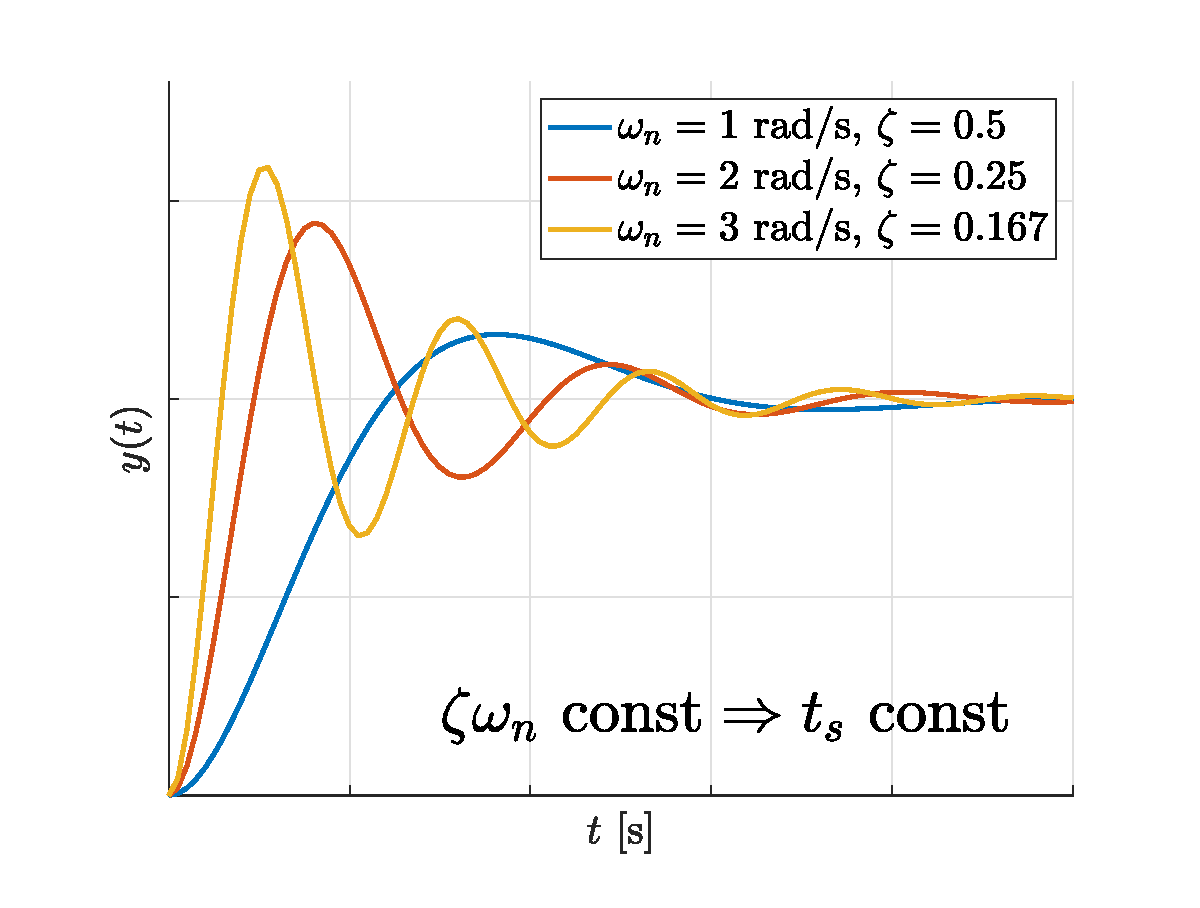
\includegraphics[scale = 0.15]{figs/4.eps}
    \end{minipage}%
    %\vrule
    \begin{minipage}{.16\textwidth}
        \centering
        \scalebox{0.5}{\input{figs/fig7}}
        \scalebox{0.5}{\begin{tikzpicture}[scale = 1]
	\draw[-latex] (-2,0) -- (0.5,0) node [below] {$\sigma$};
	\draw[-latex] (0,-2) -- (0,2) node [left] {$j\omega$};
	
	\foreach \Point in {(-0.5,1), (-0.5,-1)}{
        \node at \Point {\textcolor{bblue}{$\pmb{\times}$}};
    }
    \foreach \Point in {(-1,1), (-1,-1)}{
        \node at \Point {\textcolor{oorange}{$\pmb{\times}$}};
    }
    \foreach \Point in {(-1.5,1), (-1.5,-1)}{
        \node at \Point {\textcolor{yyellow}{$\pmb{\times}$}};
    }
    \draw[dashed] (-1.8,1) -- (0.25,1);
    \draw[dashed] (-1.8,-1) -- (0.25,-1);
\end{tikzpicture}}
    \end{minipage}%
    \begin{minipage}{.34\textwidth}
        \centering
        \includegraphics[scale = 0.15]{figs/3.eps}
        \includegraphics[scale = 0.15]{figs/5.eps}
    \end{minipage}
    
    Assim, $\zeta \uparrow \ \Rightarrow S\% \downarrow$, $\omega_d \uparrow \ \Rightarrow t_p \downarrow$ e $\zeta\omega_n \uparrow \ \Rightarrow t_s \downarrow$\\
    
    Para sistemas de fase não mínima, pelo menos um pólo e/ou zero no s.p.c.d. tem-se:
    \begin{itemize}
        \item pólo -- instabilidade
        \item zero -- derivada da resposta a $u(t)$ negativa na origem 
    \end{itemize}
    
    Pode desprezar-se o pólo real não dominante quando o regime transitório é desprezável ao fim de 5 constantes de tempo ou quando o módulo do pólo é pelo menos 5 vezes maior que o dos outros.
\end{cheatsheetbox}

\begin{cheatsheetbox}{Estabilidade}{0.0cm}
    Critério de Hurwitz: Num sistema de 1ª e 2ª ordem, é condição necessária e suficiente para o sistema ser estável que os coeficientes do polinómio denominador sejam todos positivos. É condição necessária (mas não suficiente) de estabilidade de um sistema de 3ª ou maior ordem que todos os coeficientes do polinómio denominador sejam positivos (ou tenham o mesmo sinal).
\end{cheatsheetbox}

\begin{cheatsheetbox}{Realimentação}{0.0cm}
    \begin{center}
        \includegraphics[scale = 0.5,  trim = 5cm 21.5cm 5.8cm 4.5cm, clip]{figs/fig10.pdf}
    \end{center}
    $Y(s) = \frac{K(s)G(s)}{1 + K(s)G(s)H(s)}R(s) + \frac{1}{1 + K(s)G(s)H(s)}D(s) - \frac{K(s)G(s)H(s)}{1 + K(s)G(s)H(s)}N(s)$ \\
    Erro em regime estacionário: $e_\text{ss} = \lim_{t \to \infty} e(t) \stackrel{\textbf{TVF}}{=} \lim_{s \to 0} sE(s)$ e $E(s) = \frac{1}{1 + K(s)G(s)H(s)}R(s)$ \\
    Erro de posição: $R(s) = \frac{1}{s} \Rightarrow e_\text{ss} = \frac{1}{1 + K_p}, \ K_p = \lim_{s \to 0} K(s)G(s)H(s)$ \\
    Erro de velocidade: $R(s) = \frac{1}{s^2} \Rightarrow e_\text{ss} = \frac{1}{K_v}, \ K_v = \lim_{s \to 0} sK(s)G(s)H(s)$ \\
    Erro de aceleração: $R(s) = \frac{1}{s^3} \Rightarrow e_\text{ss} = \frac{1}{K_a}, \ K_a = \lim_{s \to 0} s^2K(s)G(s)H(s)$
\end{cheatsheetbox}

\begin{cheatsheetbox}{Root Locus}{0.0cm}
    Se $s$ é pólo da f.t.c.f. então $1 + K(s)G(s)H(s) = 0$
    \begin{itemize}
        \item Condição de módulo: $|K(s)G(s)H(s)| = 1$
        \item Condição de argumento: $\arg\left[K(s)G(s)H(s)\right] = (2 \gamma + 1)180^\circ, \ \gamma \in \mathbb{Z}$
    \end{itemize}
    
    \textbf{Construção:}
    \begin{enumerate}
        \item Identificar nº zeros/pólos $(m, n)$ da f.t.c.a -- $K(s)G(s)H(s)$. O número de ramos do root locus é igual a $n$ e este é simétrico em relação ao eixo real
        \item Agrupar 2 a 2 cada par de elementos subsequente que pertença ao eixo real -- $n$ agrupamentos
        \item O root locus parte ($k = 0$) de pólos para zeros, $m$ ramos tendem para os zeros da f.t.c.a. e $n - m$ ramos tendem para o infinito (módulo)
        \item Assíntotas: $\sigma_a = \frac{\sum \text{pólos}_\text{f.t.c.a.} - \sum \text{zeros}_\text{f.t.c.a.}}{n - m}$ e $\phi_a = \frac{(2\gamma + 1)180^\circ}{n - m} \rightarrow n - m$ assíntotas
    \end{enumerate}
\end{cheatsheetbox}

\begin{cheatsheetbox}{Root Locus (cont.)}{0.0cm}
    \begin{enumerate}
        \setcounter{enumi}{4}
        \item Pontos de entrada e saída (interseção com o eixo real): escrever $1 + K(s)G(s)H(s) = 0$ em ordem a $k$ e resolver $\frac{dk}{ds} = 0$. Os mínimos relativos são pontos de entrada e os máximos relativos de saída
        \item Interseção com o eixo imaginário: resolver $1 + K(s)G(s)H(s) = 0$ em ordem a $s = j\omega$
        \item Calcular valor $k^*$ limite para a estabilidade: escrever $1 + K(s)G(s)H(s) = 0$ em ordem a $k$ e resolver para as soluções do ponto anterior
    \end{enumerate}
\end{cheatsheetbox}

\begin{cheatsheetbox}{Diagrama de Bode}{0.0cm}
    \begin{center}
        \includegraphics[scale = 0.66, trim = 4.2cm 10.9cm 4.2cm 2cm, clip]{figs/fig11.pdf} \\
    
        $G_\text{M} = \frac{1}{|G(j\omega_{180^\circ})|} \qquad P_\text{M} = \arg\left[G(j\omega_{0 \text{dB}})\right] + 180^\circ$
    \end{center}
    
    \textbf{Bons valores:} $G_\text{M} > 6 \ \text{dB} \qquad 30^\circ < P_\text{M} < 60^\circ$
    
    Para sistemas de 2ª ordem: 
    
    $P_\text{M} = 90^\circ - \arctan\left(\frac{\sqrt{-2\zeta^2 + \sqrt{4\zeta^4 + 1}}}{2 \zeta}\right)$
\end{cheatsheetbox}

\begin{cheatsheetbox}{Critério de Nyquist}{0.0cm}
    \begin{minipage}{0.4\textwidth}
        \hspace{-0.5cm}
        \scalebox{0.85}{\begin{tikzpicture}[scale = 1]
	\draw[-latex] (-0.5,0) -- (2,0) node [below] {};
	\draw[-latex] (0,-2) -- (0,2) node [left] {};
	\draw[bblue, very thick] (0,1.5) arc (90:-90:1.5);
	\draw[bblue, very thick] (0,0.5) arc (90:-90:0.5);
	\draw[bblue, very thick] (0, -1.5) -- (0, -0.5);
	\draw[bblue, very thick] (0, 1.5) -- (0, 0.5);
	\node [bblue] at (1.7, 1.5) {contorno $A$};
	\node [] at (-0.4, 1) {$j\infty$};
	\node [] at (-0.5, -1) {$-j\infty$};
	\node [bblue] at (0.7, 0.2) {$s_0$};
	\node [] at (-0.2, 0.25) {$\varepsilon$};
	\node [] at (0.9, -0.25) {$\infty$};
	\draw [->, dashed, thick] (0,0) -- (1.3,-0.75);
	\draw [->, dashed, thick] (0,0) -- (0.25,0.433);
	
    \foreach \Point in {(0, 1), (0, -1)}{
        \node at \Point {\textcolor{bblue}{\rotatebox[origin=c]{90}{$\pmb{>}$}}};
    }
    
    \foreach \Point in {(0.354, -0.354)}{
        \node at \Point {\textcolor{bblue}{\rotatebox[origin=c]{45}{$\pmb{>}$}}};
    }
    \foreach \Point in {(0.354, 0.354)}{
        \node at \Point {\textcolor{bblue}{\rotatebox[origin=c]{135}{$\pmb{>}$}}};
    }
    \foreach \Point in {(1.061, -1.061)}{
        \node at \Point {\textcolor{bblue}{\rotatebox[origin=c]{45}{$\pmb{<}$}}};
    }
    \foreach \Point in {(1.061, 1.061)}{
        \node at \Point {\textcolor{bblue}{\rotatebox[origin=c]{135}{$\pmb{<}$}}};
    }
    \foreach \Point in {(0.5, 0)}{
        \node at \Point {\textcolor{bblue}{\textbullet}};
    }
\end{tikzpicture}} \\
        \footnotesize Caso a f.t.c.a. não tiver pólos na origem faz-se $\varepsilon = 0$, caso contrário faz-se $\varepsilon \to 0$
    \end{minipage}%
    \hspace{-0.5cm}
    \begin{minipage}{0.65\textwidth}
        \begin{center}
            $\boxed{Z = N + P}$
        \end{center}
        \begin{itemize}
            \item $Z$ -- nº de zeros de $1 + K(s)G(s)H(s)$ no interior do contorno $A$
            \item $P$ -- número de pólos da f.t.c.a. no interior do contorno $A$
            \item $N$ -- número de voltas no sentido dos ponteiros do relógio da f.t.c.a. em torno de $-1$
        \end{itemize}
    \end{minipage}
    \\
    \begin{center}
        $\boxed{\text{Estabilidade da f.t.c.f.} \Leftrightarrow Z = 0 \Leftrightarrow -N = P}$
    \end{center}
    Quando a f.t.c.a. tem $k$ pólos/zeros no s.p.c.d. e 1 pólo na origem, através do contorno $A$ representado. Se $k$ for \textbf{ímpar}, as contribuições para $\arg(s_0)$ somam $180^\circ$ e portanto para $re^{j\theta}$ com $r \to 0^+$ o contorno de Nyquist fecha pela \textbf{esquerda}. Se $k$ for \textbf{par}, as contribuições para $\arg(s_0)$ somam $0^\circ$ e portanto o contorno de Nyquist fecha pela \textbf{direita}. \\
    
    Nem sempre a estabilidade da f.t.c.f. é sinónimo de $G_\text{M} > 0 \ \text{dB}$ e $P_\text{M} > 0^\circ$. Só se $Z = 0$!
    \begin{itemize}
        \item Para sistemas de 1ª e 2ª ordens, em que não existe cruzamento do diagrama de Nyquist com o semi-eixo real negativo, $G_\text{M} = \infty$
        \item Para sistemas de ordem superior pode haver mais do que um ponto de cruzamento do diagram de Nyquist com o semi-eixo real negativo
        \item Sistemas em cadeia aberta de fase não mínima
    \end{itemize}
    
    Aplicando um atraso $\tau$ a uma f.t.c.f. estável, a novas margens serão: $G'_\text{M} = G_\text{M}$ e $P'_\text{M} = P_\text{M} - \omega_{0 \text{dB}}\tau$. O intervalo de atrasos para o qual a f.t.c.f. se mantém estável é $\tau \in [0, \tau^*[$, onde $\tau^* = \frac{P_\text{M}}{\omega_{0 \text{dB}}}$
    
    \begin{minipage}{0.5\textwidth}
        $G_\text{M} = 20\log_{10}(a)$ \\
        $P_\text{M} = \alpha$
    \end{minipage}%
    \begin{minipage}{0.5\textwidth}
        \centering
        \includegraphics[scale = 0.8, trim = 9cm 23.5cm 9cm 2.2cm clip]{figs/fig13.pdf}
    \end{minipage}
    
    \textbf{Útil:} $\tan(\alpha + \beta) = \frac{\tan(\alpha) + \tan(\beta)}{1 - \tan(\alpha)\tan(\beta)} \\ \text{\ \ \ \ \ \ \ \ } \arctan(-x) = -\arctan(x)$
\end{cheatsheetbox}

\begin{cheatsheetbox}{Loop Shaping}{0.0cm}
    \begin{itemize}
        \item Seguir a referência $r(t)$ com erro $e(t)$ $\leq -\alpha$ dB $\Leftrightarrow |K(s)G(s)| \geq \alpha$ dB
        \item Atenuar o ruído $n(t)$ de pelo menos $-\alpha$ dB $\Leftrightarrow |K(s)G(s)| \leq -\alpha$ dB
        \item Atenuar distúrbios $d(t)$ de pelo menos $-\alpha$ dB $\Leftrightarrow |K(s)G(s)| \geq \alpha$ dB
    \end{itemize}
\end{cheatsheetbox}

\small
\raggedleft
Baseado no formulário de Henrique Alves Pocinho -- 99952 \\
e Maria Madalena Barros -- 100026 \\
Transcrito, editado e adaptado por \\
João Marafuz Gaspar -- 96240 \\
IST, 2022

\end{multicols}

\end{document}

